% \section*{Mô hình sinh cử chỉ OHGesture}

% \section*{3 Phương Pháp Của Chúng Tôi}
% Diffusion là mô hình đằng sau các thành công của  Stable Diffusion, Midjourney và DALL-E trong việc tạo ra các tấm ảnh siêu thực.


%. Biếm tiềm ẩm ở đây là cử chỉ và điều kiện là cảm xúc. 
%Kiến trúc của OHGesture được trình bày như hình \autoref{fig:diffusion_forward}.


\section{Mô hình của đề xuất OHGesture}
\label{sec:ohgesture}

\begin{figure}
	\centering
	\includegraphics[width=\linewidth]{images/diffusion_forward}
	\caption{Minh hoạ quá trình khử nhiễu (denoising) cử chỉ}
	\label{fig:diffusion_forward}
\end{figure}

Mô hình \textbf{OHGesture} của chúng tôi áp dụng mô hình khuếch tán \cite{ho2020denoising} với điều kiện \cite{ho2022classifier} (Classifier-Free Diffusion Guidance). Trong đó $x_0$ là chuỗi cử chỉ $g \in \mathbb{R}^{N \times 1141}$, với điều kiện $c$bao gồm  .
Với đầu vào bao gồm cử chỉ khởi tạo $x_{\text{seed}}$, âm thanh $a$ và văn bản $t$.
% với biến tiềm ẩn   (diffusion latent variable)
Mô hình diffusion bao gồm hai quá trình: quá trình tạo nhiễu (diffusion) $q$ và quá trình khử nhiễu (denoising process) $p_{\theta}$. 
Trước tiên chúng tôi trình bày trước về phương pháp nền tảng (baseline) của mô hình diffusion.

\subsection{Quá trình trích xuất đặc trưng}

Dữ liệu để học của chúng tôi được lấy từ tập dữ liệu BEAT (Body-Expression-Audio-Text)
\cite{liu2022beat}. Tương tự mô hình DiffuseStyleGesture \cite{yang2022DiffuseStyleGestureplus} chúng tôi cũng sử dụng đầu vào bao gồm âm thanh, cử chỉ và cảm xúc, ngoài ra chúng tôi sử dụng thêm dữ liệu văn bản.

\begin{itemize}
	\item \textbf{Cử chỉ}: Cử chỉ ground truth là dữ liệu bao gồm 75 khớp xương được trình bày ở công thức \ref{eq:gesturevector}. Chúng tôi cắt $N_{\text{seed}} = 8$ frame đầu để làm cử chỉ khởi tạo và $N$ frame tiếp theo làm cử chỉ để dự đoán theo âm thanh và văn bản.
	
%	\item\textbf{Âm thanh}: Âm thanh sẽ được dùng làm đặc trưng để sinh cử chỉ, Chúng tôi sử dụng các mô hình Pretrain có sẵn như WavLM \cite{chen2022wavlm} để trích xuất đặc trưng âm thanh. 
%	Chúng tôi kết hợp thêm các đặc trưng về MFCC, Mel-Spectrum, Pitch, Enery và Onsets \cite{bello2005tutorial}
  \item \textbf{Âm thanh}: Tất cả dữ liệu âm thanh được giảm số sample rate (downsampled) xuống $16 \mathrm{kHz}$ và các vector tiềm ẩn được lấy từ các mô hình pre-train của WavLM Large \cite{chen2022wavlm}. Chúng tôi sử dụng nội suy tuyến tính (interpolation) để căn chỉnh đặc trưng của vector tiềm ẩn trong WavLM và cử chỉ $x_{0}$ theo chiều thời gian thành $20fps$, sau đó sử dụng một lớp tuyến tính để giảm kích thước của đặc trưng xuống còn 64 tạo thành chuỗi đặc trưng âm thanh cuối cùng $\mathbf{A}$.
		
	\item \textbf{Cảm xúc}: Cảm xúc bao gồm 6 cảm xúc khác nhau được biểu diễn thành một vector theo phương pháp one-hot encoding.
	
	\item \textbf{Văn bản}: Văn bản được trích xuất thông qua mô hình FastText \cite{yoon2022genea} để lấy được vector word embedding.
	
	\item \textbf{Cử chỉ nhiễu} (Noisy gesture): khi huấn luyện, $x_{t}$ là cử chỉ nhiễu có cùng kích thước như cử chỉ gốc $x_{0}$ sẽ được sinh ngẫu nhiên từ phân phối chuẩn $\mathcal{N}(0, \mathbf{I})$. Khi sinh ngẫu nhiên, cử chỉ nhiễu ban đầu $x_{T}$ được lấy mẫu từ phân phối chuẩn tiêu chuẩn và các $x_{t}, t<T$ khác là kết quả của bước làm nhiễu trước đó. Sau đó, kích thước được điều chỉnh thành 256 như $\mathbf{G}$ bằng lớp linear.
	
\end{itemize}

%\item Bước làm nhiễu: Trong quá trình huấn luyện, bước làm nhiễu $t$ được lấy mẫu từ phân phối chuẩn của $\{1,2, \ldots, T\}$, với mã hóa vị trí (position encoding) giống như mô hình Transformer \cite{vaswani2017attention}, sau đó được ánh xạ vào không gian $\mathbf{T}$ có kích thước 256 bằng một mạng perceptron nhiều lớp (MLP).
%
%
%
%\item Cảm xúc: Các cảm xúc của cử chỉ được biểu diễn dưới dạng vectơ one-hot encoding, tức thành vector toàn bộ là số $0$ và vị trí có cảm xúc tương ứng có vị trí là $1$, vector one-hot encoding được ánh xạ vào không gian có kích thước 64 $\mathbf{S}$ thông qua một lớp tuyến tính.
%
%\item Cử chỉ khởi tạo: Cử chỉ khởi tạo giúp tạo ra sự chuyển tiếp mượt mà giữa các lần sinh liên tiếp \cite{yoon2020speech}. Cử chỉ khởi được cắt ngắn xuống $g \in$ $\mathbb{R}^{(8+N) \times 1141}$. Trong quá trình training, $8$ frame đầu tiên của cử chỉ $g$ được sử dụng làm cử chỉ khởi tạo $d$ và $N$ frame còn lại được sử dụng làm cử chỉ thật $x_{0}$ để tính hàm loss $\mathcal{L}$. Sau đó, chúng tôi ánh xạ các đặc trưng của cử chỉ khởi tạo $d$ vào không gian $\mathbf{D}$ có kích thước $192$ chiều bằng một lớp tuyến tính. 
%Kết quả cử chỉ được sinh ra trong $4$ giây, và vì cử chỉ sinh ra được chạy ở $20 \mathrm{fps}$ (tương đương 20 khung hình mỗi giây) nên kích thước $N=80$.

%\section{Mô hình diffusion cho bài toán sinh cử chỉ}

\begin{figure}
	\centering
	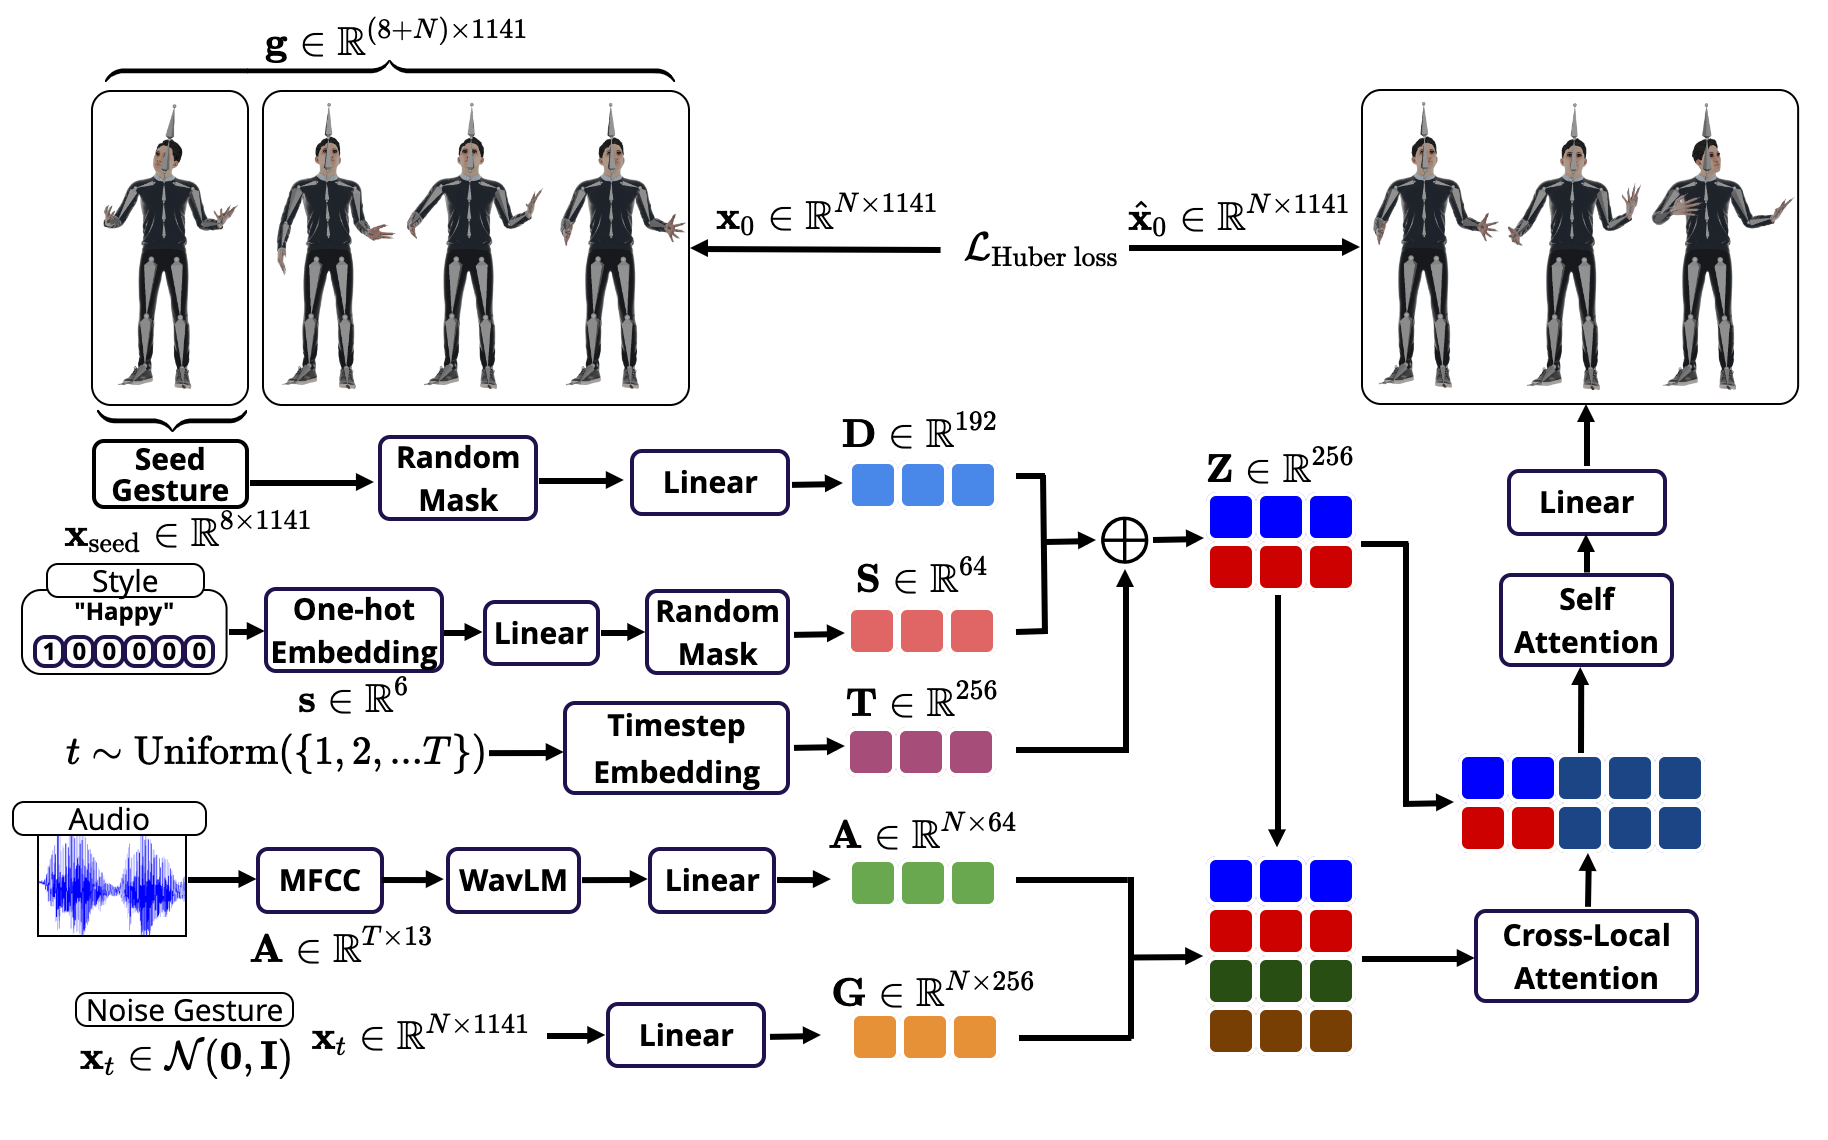
\includegraphics[width=\linewidth]{images/architecture_diffusion}
	\caption{Kiến trúc OHGesture}
	\label{fig:architecturediffusion}
\end{figure}


% Ý tưởng của chúng tôi là tạo ra các cử chỉ bằng một mô hình diffusion \cite{ho2020denoising} bằng cách học cách dần dần Denoise từ nhiễu hoàn toàn. Như được thể hiện trong Hình 2, mô hình diffusion bao gồm hai phần: quá trình tiến lùi (quá trình diffusion)  và quá trình ngược lại (quá trình Denoise).

%\subsection{Quá Trình Gây Nhiễu (Diffusion)}
%
%Quá trình diffusion $q$ được mô hình hóa như là một quá trình Markov với đầu vào lần lượt được thêm nhiễu, và sau đó mô hình lần lượt từng bước học để có thể tái tạo lại cử chỉ ban đầu.
%Trong bài toán sinh cử chỉ, đầu vào là các điểm trên tọa độ 3D, gọi là keypoint $x$, với $x_{0} \sim q\left(x_{0}\right)$ và $q\left(x_{0}\right)$ là phân phối của dữ liệu thực tế.
%Trong đó mỗi bước phương sai được thay đổi theo hệ số $\beta_{1}, \beta_{2}, \ldots, \beta_{T}$ $\left(0<\beta_{1}<\beta_{2}<\cdots<\beta_{T}<1, T\right)$, chúng tôi thêm nhiễu Gaussian
%
%\begin{equation} \label{eq:gaussian}
%q\left(x_{t} \mid x_{t-1}\right)=\mathcal{N}\left(x_{t} ; \sqrt{1-\beta_{t}} x_{t-1}, \beta_{t} \mathbf{I}\right)
%\end{equation}
%
%vào cử chỉ tại mỗi thời điểm $t$ lần lượt, và sau khi nhiễu Guassian được thêm vào đến bước $T$ đủ lớn, đến khi kết quả trở nên nhiễu hoàn toàn và không thể phân biệt được với kết quả ban đầu.

%\subsection{Quá Trình Khử Nhiễu (Denoise)}
%
%Quá trình Denoise $p_{\theta}$ là quá trình học tham số $\theta$ thông qua một mạng neural. Giả sử quá trình Denoise cũng tuân theo phân phối Gaussian, tức là nhiễu $x_{t}$ tại thời điểm $t$ được sử dụng để học $\mu_{\theta}, \Sigma_{\theta}$, sau đó
%
%\begin{equation} \label{eq:diffusion}
%p_{\theta}\left(x_{t-1} \mid x_{t}\right)=\mathcal{N}\left(x_{t-1} ; \mu_{\theta}\left(x_{t}, t\right), \Sigma_{\theta}\left(x_{t}, t\right)\right)
%\end{equation}
%
%Để thuận tiện cho việc tính toán, ta cho $\alpha_{t}=1-\beta_{t}$ và viết gọn lại $\bar{\alpha}_{t}=\prod_{i=1}^{T} \alpha_{i}$. Sau đó, cử chỉ nhiễu $x_{t}$ tại thời điểm $t$ có thể được viết lại như sau:
%
%\begin{equation} \label{eq:denoisevariance}
%q\left(x_{t} \mid x_{0}\right)=\mathcal{N}\left(x_{t} ; \sqrt{\bar{\alpha}_{t}} x_{0},\left(1-\bar{\alpha}_{t}\right) \mathbf{I}\right)
%\end{equation}
%
%Mô hình học bằng cách tối ưu hóa bằng cách giảm thiểu sự khác biệt giữa nhiễu thực sự $\epsilon$ và nhiễu được dự đoán $\epsilon_{\theta}\left(x_{t}, t\right)$ \cite{ho2020denoising}. Khi lấy mẫu, chúng ta có thể học giá trị trung bình $\mu_{\theta}\left(x_{t}, t\right)=\frac{1}{\sqrt{\alpha_{t}}}\left(x_{t}-\frac{\beta_{t}}{\sqrt{1-\bar{\alpha}_{t}}} \epsilon_{\theta}\left(x_{t}, t\right)\right)$ với phương sai cố định.

\subsection{Sinh cử chỉ với điều kiện}

Mục tiêu của chúng tôi là tổng hợp một cử chỉ con người $x^{1: N}$ có độ dài $N$ dựa trên điều kiện $c$. Trong mô hình OHGesture, tương tự như các phương pháp \cite{ramesh2022hierarchical} \cite{tevet2022human}, chúng tôi dự đoán dự liệu thật thay vì dự đoán nhiễu $\epsilon_{\theta}\left(x_{t}, t\right)$ như \cite{ho2020denoising}. Quá trình khử nhiễu (Denoise) tái tạo dữ liệu gốc $x_{0}$ dựa trên nhiễu đầu vào $x_{t}$, bước làm nhiễu $t$ và điều kiện $c$

\begin{equation} \label{eq:condition}
\hat{x}_{0}=\text { Denoise }\left(x_{t}, t, c\right)
\end{equation}

Sau đó, hàm khử nhiễu có thể được huấn luyện bằng cách tối ưu hóa hàm Huber loss \cite{huber1992robust} giữa các cử chỉ dự đoán $\hat{x}_{0}$ và các cử chỉ thực tế $x_{0}$ trên các tập huấn luyện:

\begin{equation} \label{eq:huberloss}
\mathcal{L}=E_{x_{0} \sim q\left(x_{0} \mid c\right), t \sim[1, T]}\left[\operatorname{HuberLoss}\left(x_{0}-\hat{x}_{0}\right)\right]
\end{equation}

\section{Áp dụng cơ chế Attention cho bài toán sinh cử chỉ}

\subsection{Hàm xử lý đặc trưng của quá trình khử nhiễu}

Như kiến trúc \textbf{OHGesture} trình bày trong hình \autoref{fig:architecturediffusion}, cử chỉ được tạo ra dựa trên bước làm nhiễu $t$, cử chỉ nhiễu $x_{t}$ và điều kiện $c$ (bao gồm âm thanh $a$, cảm xúc $s$ và cử chỉ khởi tạo $d$ ). Đối với mỗi đặc trưng, quá trình sinh cử chỉ được xử lý như sau:


\subsection{Cơ chế Attention trong hàm khử nhiễu}

Chúng tôi thực hiện việc khử nhiễu với kiến trúc dựa trên cơ chế attention. Để tính được tương quan của các đặc trưng xa, chúng tôi sẽ học để biểu diễn được các ngữ cảnh cực bộ (local context) theo \cite{rae2020transformers}.

Đầu tiên cử chỉ khởi tạo $\mathbf{D}$ và vector cảm xúc $\mathbf{S}$ được ghép lại với nhau để tạo thành một vectơ có kích thước 256, sau đó thêm vector làm nhiễu $\mathbf{T}$ để tạo thành vector $\mathbf{Z}$. 
Sau đó, vectơ $\mathbf{Z}$ và các bản sao của nó được ghép thành một chuỗi vector đặc trưng để khớp với dòng thời gian của âm thanh và đặc trưng cử chỉ, sau đó ghép với âm thanh $\mathbf{A}$ và cử chỉ $\mathbf{G}$ để làm đầu vào cho lớp local attention (chú ý cục bộ). 
Phương pháp sinh cử chỉ song hành với âm thanh của chúng tôi sử dụng lớp Local Attention được lấy ý tưởng từ phương pháp Routing Transformer \cite{roy2021efficient}, mà cho thấy rằng local attention quan trọng trong việc xây dựng biểu diễn trung gian, như được thể hiện trong Hình 3(c).

Sau đó, chúng tôi nối đầu ra của lớp local attention với $\mathbf{Z}$ và đưa vào lớp self-attention, như được thể hiện trong \autoref{fig:architecturediffusion}. Cơ chế self-attention tương tự như trình mã hóa (encoding) của Transformer \cite{vaswani2017attention}, giúp tính toán được mối liên hệ giữa các chuỗi dữ liệu với công tức sau:


\begin{equation} \label{eq:attention}
\operatorname{Attention}(\mathbf{Q}, \mathbf{K}, \mathbf{V}, \mathbf{M})=\operatorname{softmax}\left(\frac{\mathbf{Q} \mathbf{K}^{T}+\mathbf{M}}{\sqrt{C}}\right) \mathbf{V}
\end{equation}

trong đó $\mathbf{Q}, \mathbf{K}, \mathbf{V}$ là vector query, key và value từ dữ liệu đầu vào và $\mathbf{M}$ là mặt nạ (mask) giúp xác định loại của cơ chế attention, bao gồm \textit{full self-attention}, \textit{sliding window attention} và \textit{cross-local attention}. Để yếu tố thời gian không ảnh hưởng nhiều đến kết quả sinh cử chỉ, chúng tôi sử dụng cơ chế mã hóa vị trí tương đối (Relative Position Encoding - RPE) được trình bày trong phương pháp Reformer \cite{kitaev2020reformer}. Cuối cùng, đầu ra của self-attention được ánh xạ lại cùng kích thước như $x_{0}$ sau một lớp biến đổi tuyến tính.

\begin{figure*}[ht]
\begin{minipage}[b]{0.25\textwidth}
\centering
    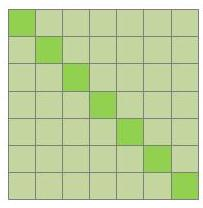
\includegraphics[width=\textwidth]{images/attention_full.jpg}
    \caption*{(a) full self-attention}
\end{minipage}
\hfill
\begin{minipage}[b]{0.25\textwidth}
\centering
    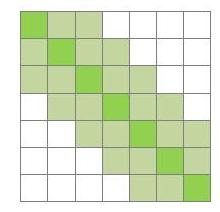
\includegraphics[width=\textwidth]{images/attention_sidewindow.jpg}
    \caption*{(b) sliding window attention}
\end{minipage}
\hfill
\begin{minipage}[b]{0.25\textwidth}
\centering
    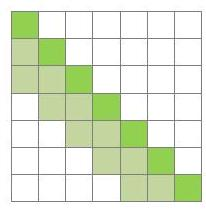
\includegraphics[width=\textwidth]{images/cross_attention.jpg}
    \caption*{(c) cross-local attention}
\end{minipage}
% \label{fig:type_attention}
\caption[Các loại attention khác nhau (full self-attention, sliding window attention, cross-local attention)]{Các loại attention khác nhau được sử dụng trong các thí nghiệm của chúng tôi, trong đó (a) và (c) là cơ chế attention được sử dụng trong mô hình của chúng tôi và (b) là một mẫu được sử dụng để đánh giá trong thực nghiệm. Mỗi dòng tương ứng với input và mỗi cột tương ứng với output của mô hình}
\end{figure*}

% Phần 4.3. Các hàng đại diện cho các đầu ra và các cột đại diện cho đầu vào. Các hình vuông màu sáng tô màu cho các phần tử liên quan đến mỗi dòng đầu ra.


Các cơ chế attention khác nhau có thể được tạo ra bằng cách điều chỉnh lớp mask tương ứng $\mathbf{M}$, 
tương tự như phương pháp Longformer \cite{beltagy2020longformer} chúng tôi cũng thử nghiệm cơ chế \textit{sliding window attention}.

\subsection{Phương pháp sample cử chỉ}

Để có thể sinh cử chỉ với chiều dài tùy ý, chúng tôi cắt chuỗi ban đầu thành các đoạn ngắn có chiều dài $N$. Trong quá trình huấn luyện, cử chỉ khởi tạo đầu tiên có thể được tạo ra bằng cách lấy ngẫu nhiên cử chỉ từ tập dữ liệu hoặc từ lấy trung bình từ đoạn cắt được. Cụ thể ở đây, sẽ lấy góc quay trung bình trong các đoạn đã cắt được. Tiếp theo chúng ta chỉ việc lấy lần lượt các frame đã sinh ra và chọn $8$ frame cuối cùng làm cử chỉ khởi tạo ở lượt tiếp theo. Đối với mỗi đoạn đã cắt ra, cử chỉ $x_{t}$ lần lượt sẽ được áp dụng hàm khử nhiều $\hat{x}_{0} = Denoise \left(x_{t}, t, c\right)$ cho đến khi được  $x_{t-1}$, và $x_{t-1}$ sẽ tiếp tục được làm khử nhiễu cho đến bước khử nhiễu $t=T$ sẽ đạt được $x_{0}$ như kiến trúc trong phần \autoref{fig:architecturediffusion}.


% chúng tôi , trong mỗi bước làm nhiễu $t$, chúng tôi dự đoán cử chỉ sạch  $=$  $\left(x_{t}, t, c\right)$, và thêm nhiễu vào bước làm nhiễu $x_{t-1}$ sử dụng Phương trình (1) với quá trình trải đều. Quá trình này được lặp lại từ $t=T$ cho đến khi đạt được $x_{0}$ (Hình 2 dưới cùng).

\section{Điều khiển cảm xúc trong bài toán sinh cử chỉ}

\begin{figure}[htbp]
    \centering
    \begin{subfigure}[b]{0.3\textwidth}
         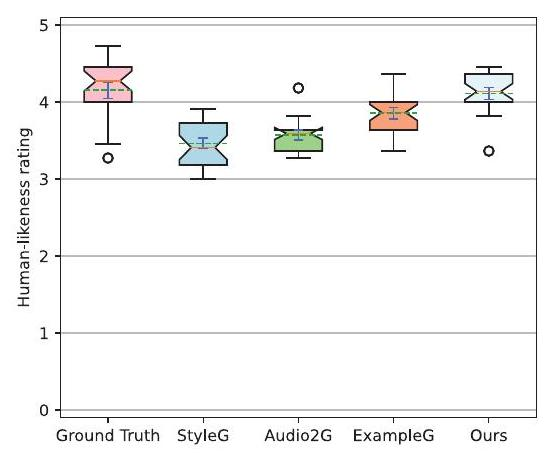
\includegraphics[width=\textwidth]{images/humanlike_score.jpg}
        \caption*{(a) Biểu đồ hộp của đánh giá về tính giống với con người}
    \end{subfigure}
    \hfill
    \begin{subfigure}[b]{0.3\textwidth}
        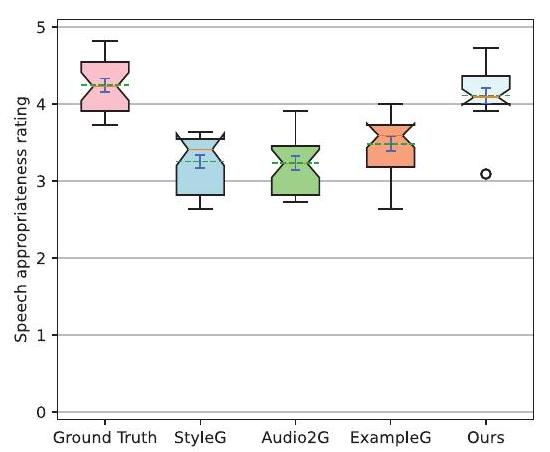
\includegraphics[width=\textwidth]{images/speech_score.jpg}
         \caption*{(b) Biểu đồ hộp của đánh giá về tính phù hợp giữa cử chỉ và âm thanh.}
    \end{subfigure}
    \hfill
    \begin{subfigure}[b]{0.3\textwidth}
        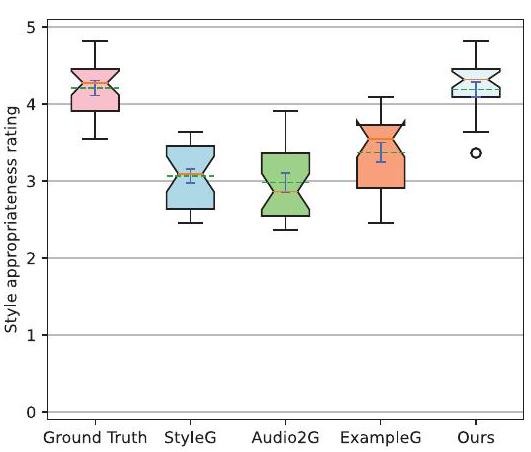
\includegraphics[width=\textwidth]{images/style_score.jpg}
        \caption*{(c) Biểu đồ hộp của đánh giá về tính phù hợp giữa cử chỉ và cảm xúc}
    \end{subfigure}
    \caption[Biểu đồ hộp mô tả kết quả so sánh MOS]{Biểu đồ hộp mô tả kết quả so sánh MOS cho các mô hình khác nhau trong các chiều khác nhau. Hộp mở rộng từ phân vị thứ nhất thấp nhất (Q1) đến phân vị thứ ba lớn nhất (Q3) của dữ liệu. Đường đỏ chỉ là giữa. Các khe nhỏ biểu thị khoảng tin cậy $95\%$ (CI) xung quanh giữa. Khi CI nhỏ hơn Q1 hoặc lớn hơn Q3, khe mở rộng ra khỏi hộp, tạo ra một hình dáng "lật" độc đáo. Chúng tôi cũng đã đánh dấu giá trị trung bình và khoảng tin cậy $95\%$ của nó trong hình với đường nét đứt màu xanh lá cây và đường dọc màu xanh lam, tương ứng.}
    \label{fig:3col}
\end{figure}


Ở các bước trên mô hình đã có thể học được cách sinh cử chỉ, nhưng để mô hình có thể học được các cảm xúc ở các tình huống khác nhau sẽ được giải quyết bằng cách tham số hóa và lần lượt thay đổi từng cảm xúc để sao cho khi thay đổi cảm xúc thì kết quả dự đoán phải có cảm xúc tương ứng.
Tham số để điều khiển ở đây là $c$, việc điều khiển ở đây không chỉ có thể là âm thanh $a$ mà còn là cảm xúc $s$ hoặc cử chỉ khởi tạo $d$, v.v. Chúng tôi tham khảo phương pháp của \cite{ho2022classifier}, \cite{tevet2022human}, bằng cách thêm một lớp mặt nạ ngẫu nhiên (random mask) trên các vector đặc trưng của cử chỉ khởi tạo $d$ và cảm xúc $s$ vào mô hình như hình minh họa \autoref{fig:architecturediffusion} để giúp kiểm soát chính xác việc mô hình có thể học được các đặc trưng ở các điều kiện khác nhau. Khi đó, mô hình chỉ việc thay đổi nhãn tương ứng với lớp mask đã lấy ngẫu nhiên để mô hình có thể tối ưu theo các điều kiện khác nhau. Khi đó hàm khử nhiễu $\text{Denoise} \left(x_{t}, t, c_{1}\right), c_{1}=[d, s, a]$ và hàm khử nhiễu mà không có điều kiện $\text{Denoise} \left(x_{t}, t, c_{2}\right), c_{2}=[\varnothing, \varnothing, a]$ sẽ được tối ưu trong quá trình huấn luyện, theo công thức

\begin{equation} \label{eq:denoise}
\hat{x}_{0 \gamma, c_{1}, c_{2}}=\gamma \text{Denoise} \left(x_{t}, t, c_{1}\right)+(1-\gamma) \text{Denoise} \left(x_{t}, t, c_{2}\right)
\end{equation}


Trong thực tế, hàm Denoise học cả phân phối có điều kiện và không có điều kiện bằng cách ngẫu nhiên phần mask $10 \%$ của các mẫu bằng các mask theo phân phối Bernoulli. Sau đó, đối với kiểu $s$ trong điều kiện, chúng ta có thể tạo ra cử chỉ được kiểm soát kiểu khi lấy mẫu bằng cách nội suy hoặc thậm chí là dự đoán hai biến thể bằng cách sử dụng $\gamma$, như $c_{1}=\left[d, s_{1}, a\right], c_{2}=\left[d, s_{2}, a\right]$

% \begin{figure*}[ht]
% \begin{minipage}[b]{0.3\textwidth}
% \centering
%     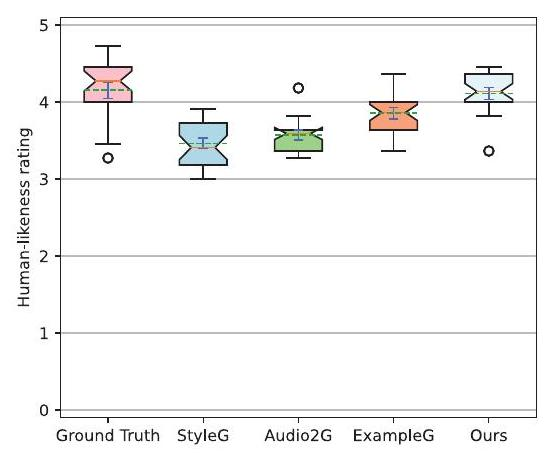
\includegraphics[width=\textwidth]{images/humanlike_score.jpg}
%     \caption*{(a) Biểu đồ hộp của đánh giá về tính giống với con người}
% \end{minipage}
% \hfill
% \begin{minipage}[b]{0.3\textwidth}
% \centering
%     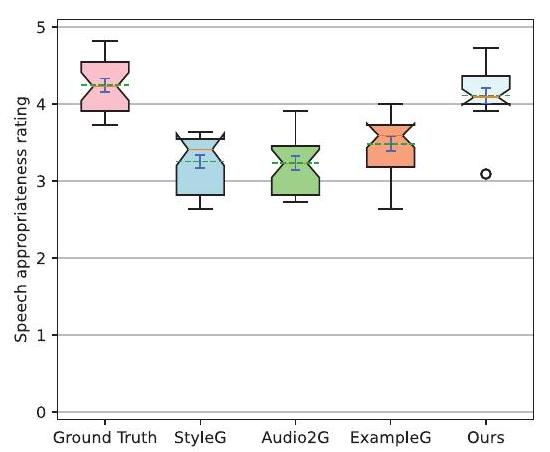
\includegraphics[width=\textwidth]{images/speech_score.jpg}
%     \caption*{(b) Biểu đồ hộp của đánh giá về tính phù hợp giữa cử chỉ và âm thanh.}
% \end{minipage}
% \hfill
% \begin{minipage}[b]{0.3\textwidth}
% \centering
%     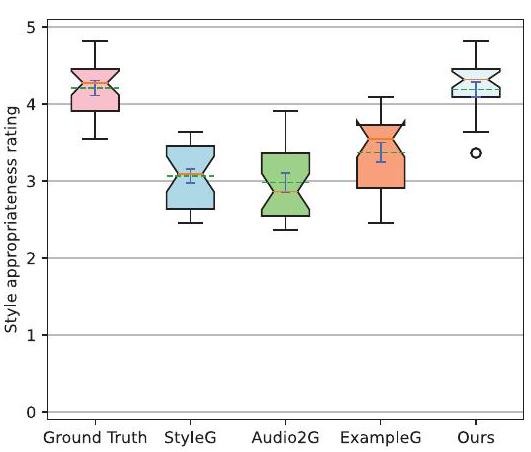
\includegraphics[width=\textwidth]{images/style_score.jpg}
%     \caption*{(c) Biểu đồ hộp của đánh giá về tính phù hợp giữa cử chỉ và cảm xúc}
% \end{minipage}
% \label{fig:gesture_score}
% \caption{Biểu đồ hộp mô tả kết quả so sánh MOS cho các mô hình khác nhau trong các chiều khác nhau. Hộp mở rộng từ phân vị thứ nhất thấp nhất (Q1) đến phân vị thứ ba lớn nhất (Q3) của dữ liệu. Đường đỏ chỉ là giữa. Các khe nhỏ biểu thị khoảng tin cậy $95\%$ (CI) xung quanh giữa. Khi CI nhỏ hơn Q1 hoặc lớn hơn Q3, khe mở rộng ra khỏi hộp, tạo ra một hình dáng "lật" độc đáo. Chúng tôi cũng đã đánh dấu giá trị trung bình và khoảng tin cậy $95\%$ của nó trong hình với đường nét đứt màu xanh lá cây và đường dọc màu xanh lam, tương ứng.}
% \end{figure*}


% Hình 4: Biểu đồ hộp thể hiện kết quả so sánh của MOS cho các mô hình khác nhau trong các chiều không gian khác nhau. Hộp mở rộng từ phần tư dưới thứ nhất (Q1) đến phần tư lớn thứ ba (Q3) của dữ liệu. Đường đỏ chỉ ra trung vị. Các rãnh biểu thị khoảng tin cậy $95 \%$ (CI) xung quanh trung vị. Khi CI ít hơn Q1 hoặc lớn hơn Q3, rãnh mở rộng ra ngoài hộp, tạo cho nó một diện mạo "lật" độc đáo. Chúng tôi cũng đã đánh dấu giá trị trung bình và CI $95\%$ của nó trong hình với một đường kẻ xanh lá cây đứt và một đường kẻ đứt màu xanh dương, tương ứng.

% \begin{equation}
% \left[\mathbf{r}_p, \mathbf{r}_r, \dot{\mathbf{r}}_p, \dot{\mathbf{r}}_r, \rho_p, \rho_r, \dot{\rho}_p, \dot{\rho}_r, g_d\right]
% \end{equation}


% Mô hình OHGesture được dựa trên mô hình QPGesture \cite{yang2023qpgesture} với nền tảng chính của phương pháp dựa trên mô hình VQ-VAE là mã hóa (encode) và giải mã (decode) dữ liệu hay nói cách khác chúng ta sẽ biểu diễn toàn bộ dữ liệu ở chiều dữ liệu thấp hơn và sau đó biểu diễn ngược trở lại kích thước ban đầu. Dữ liệu được biểu diễn thành các vùng trong không gian, với mỗi vùng có một đại diện tương ứng. Từ các địa diện ta có thể mã hóa ngược trở lại để chọn ra các ứng viên cử chỉ theo ngữ nghĩa (dữ liệu văn bản) hoặc nhịp điệu lời nói (dữ liệu âm thanh).
% Dựa trên hai cử chỉ ứng viên (gesture candidate), ta trích xuất ra pha dựa trên vận tốc xoay của các các khớp khi di chuyển và dựa trên pha hiện tại của cử chỉ khởi tạo, ta sẽ chọn được cử chỉ có pha gần nhât hay phù hợp nhất để chọn ra chuỗi cử chỉ cuối cùng.

% Cụ thể quá trình huấn luyện của mô hình bao gồm các quá trình như sau: Lượng tử hóa (Quantization), Ghép các chuyển động cử chỉ (Motion Matching), Điều hướng dựa theo pha của cử chỉ (Phrase Guided).

% Kiến trúc mô hình được trình bày minh họa trong hình \autoref{fig:architecturediffusion}.








% \subsection{Lượng tử hóa (Quantization)}
% % Learning a discrete latent space representation

% Lượng tử hóa là việc học để biểu diễn dữ liệu trong không gian rời rạc (discrete latent space representation). Ta sẽ biểu diễn dữ liệu lên không gian tiềm ần (latent space).
% Mục tiêu của việc lượng tử hóa là biểu diễn dữ liệu dưới số chiều thấp hơn hay chấm điểm/đánh giá dựa trên các đặc trưng của dữ liệu, từ đó dùng các điểm đã đánh giá để so sánh với nhau. Sau khi so sánh đánh giá, ta chọn được một ứng viên tốt nhất, từ ứng viên tốt nhất ta sẽ học để giải mã (decode) ngược trở lại dữ liệu ban đầu.

% Dữ liệu đầu vào được lượng tử hóa bao gồm âm thanh, cử chỉ và văn bản. Trong bài toán sinh cử chỉ, chúng tôi chỉ tập trung vào việc xử lý dữ liệu dựa trên cử chỉ nên đôi với dữ liệu văn bản và âm thanh, ta chỉ sử dụng lại các mô hình pre-train có sẵn. Với âm thanh chúng tôi sử dụng mô hình VQ-Wave2Vec \cite{baevski2019vq} để biểu diễn các dữ liệu âm thanh thành các latent vector. Hàm lượng tử hóa âm thanh là hàm $f_{quant\_audio} : \mathbf{A} \mapsto \mathbf{Z_{audio}}$ trong đó $\textbf{A}$ là các chuỗi các âm thanh sẽ được mã hóa lên vector lantent $\textbf{Z}$. Với $\textbf{Z_{audio}} \in \mathcal{Z}_a$.

% Đối với văn bản, chúng tôi sử dụng mô hình Sentene BERT \cite{reimers2019sentence} để biểu diễn các dữ liệu văn bản thành các vector tiềm ẩn. Hàm để nhúng các dữ liệu văn bản thành các vector là hàm $f_{embedding\_text} : \mathbf{T} \mapsto \mathbf{Z_{text}}$.

% Với cử chỉ, mô hình dựa trên kiến trúc của mô hình VQ-VAE. Hàm lượng tử hóa cử chỉ là hàm $f_{quant\_gesture} : \mathbf{G} \mapsto \mathbf{Z_{gesture}}$ với $\textbf{G}$ là các vector trong codebook $\mathcal{Z_g}$

% % Sau đó dựa trên các điểm dữ liệu trước đó để tìm được đại diện phù hợp trong các vùng.
% % Dựa trên chuỗi các dữ liệu đại diện ta có thể tìm được chuỗi các pha của cử chỉ và từ đó chọn ra điểm dữ liệu cuối cùng dựa trên pha của văn bản hoặc âm thanh.

% \subsubsection{Hàm lượng tử hóa cử chỉ (Gesture Quantization)}

% Trong $f_{quant\_gesture}$ các điểm dữ liệu được phân tách và gom nhóm thành các vùng khác nhau trong không gian, với một đại diện để biểu diễn cho mỗi vùng được gọi là \textit{code} là một vector $\textbf{z} \in \mathbb{R}$. Tập các vector đại diện cho các vùng được gọi là \textit{codebook} $\mathbf{Z} \in \mathbb{R}^{D_g \times C}$ là một từ điển được biểu thị dưới dạng một ma trận bao gồm tập nhiều codebook, với mỗi code $\textbf{z} \in \mathbb{R}^C$ và $D_g$ là số lượng phần tử của codebook.

% $$
% f_{encoder} : \mathbf{X} \mapsto \mathbf{Z} \quad \quad
% f_{quantize} : \mathbf{Z} \mapsto \hat{\mathbf{Z}} \quad \quad
% f_{decoder} : \hat{\mathbf{Z}} \mapsto \mathbf{C}
% $$

% $$
% \mathcal{L}=\mathcal{L}_{\text {recontruct }}\left(\mathbf{c}, \mathbf{x}\right)+\left\|\operatorname{sg}[\mathbf{z}]-\mathbf{z}_{\mathbf{q}}\right\| +\beta\left\|\mathbf{z}-\operatorname{sg}\left[\mathbf{z}_{\mathbf{q}}\right]\right\|
% $$

% Loss function:
% $$
% \mathcal{L}_{\text {gesture }\left(E_{g}, D_{g}, \mathcal{Z}_{g}\right)}=\mathcal{L}_{\text {rec }}\left(\hat{\mathbf{G}}_{1}, \mathbf{G}\right)+\left\|\operatorname{sg}[\mathbf{g}]-\mathbf{g}_{\mathbf{q}}\right\| +\beta\left\|\mathbf{g}-\operatorname{sg}\left[\mathbf{g}_{\mathbf{q}}\right]\right\|
% $$

% Loss recontruction:

% $$
% \mathcal{L}_{r e c}\left(\hat{\mathbf{G}}_{1}, \mathbf{G}_{1}\right)=\left\|\hat{\mathbf{G}_{1}}-\mathbf{G}_{1}\right\|_{1}+\alpha_{1}\left\|\hat{\mathbf{G}}_{1}{ }^{\prime}-\mathbf{G}_{1}^{\prime}\right\|_{1} +\alpha_{2}\left\|\hat{\mathbf{G}}_{1}{ }^{\prime \prime}-\mathbf{G}_{1}^{\prime \prime}\right\|_{1}
% $$

% \subsubsection{Quantization Audio}


% $
% \mathbf{g}_{\mathbf{q}, i}=\mathcal{Q_g}(\mathbf{g})=\arg \min _{\mathbf{z}_{j} \in \mathcal{Z}_{g}}\left\|\mathbf{g}_{i}-\mathbf{z}_{j}\right\|
% $

% $
% \hat{\mathbf{G}}_{1}=\mathcal{D}_{g}\left(\mathbf{g}_{\mathbf{q}}\right)=\mathcal{D_g}\left(\mathcal{Q_g}\left(\mathcal{E_g}(\mathbf{G})\right)\right)
% $

% $
% \mathcal{L}=\sum_{k=1}^K \mathcal{L}_k^{\text {wav2vec }}+\left(\|\operatorname{sg}(\mathbf{z})-\hat{\mathbf{z}}\|^2+\gamma\|\mathbf{z}-\operatorname{sg}(\hat{\mathbf{z}})\|^2\right)
% $

% $
% \mathcal{L}_k^{\text {wav2vec }}=-\sum_{i=1}^{T-k}\left(\log \sigma\left(\mathbf{z}_{i+k}^{\top} h_k\left(\mathbf{c}_i\right)\right)+\underset{\tilde{\mathbf{z}} \sim p_n}{\mathbb{E}}\left[\log \sigma\left(-\tilde{\mathbf{z}}^{\top} h_k\left(\mathbf{c}_i\right)\right)\right]\right)
% $


% \section{Motion Matching}
% $
% \hat{\mathbf{C}}_{a}=\left\{\hat{\mathbf{C}}_{a}^{0}, \hat{\mathbf{C}}_{a}^{1}, \ldots, \hat{\mathbf{C}}_{a}^{C_{b}}\right\}
% $

% $
% \hat{\mathbf{C}}_{g}=\left\{\hat{\mathbf{C}}_{g}^{0}, \hat{\mathbf{C}}_{g}^{1}, \ldots, \hat{\mathbf{C}}_{g}^{C_{b}}\right\}
% $

% $
% \hat{\mathbf{C}}_{t}=\left\{\hat{\mathbf{C}}_{t}^{0}, \hat{\mathbf{C}}_{t}^{1}, \ldots, \hat{\mathbf{C}}_{t}^{C_{b}}\right\}
% $



% \subsection{Phrase Guidance}

% \begin{figure}
%     \centering
%     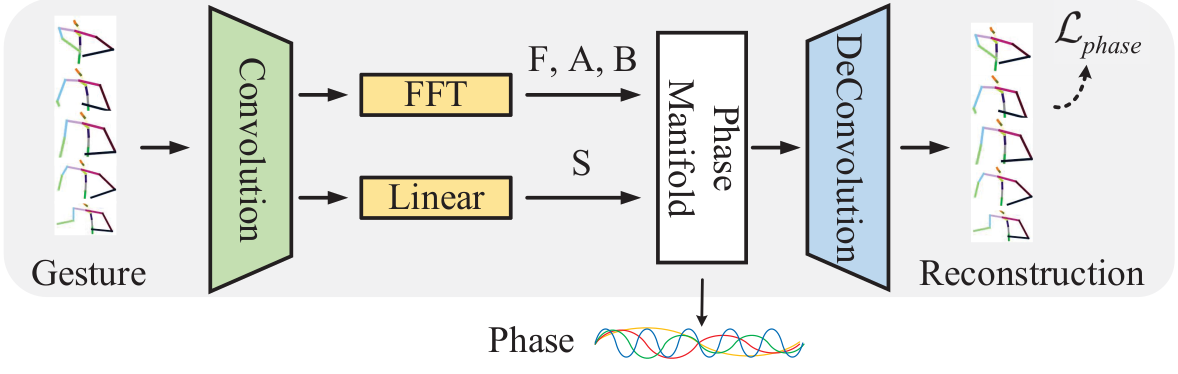
\includegraphics[width=\linewidth]{images/phrase_guidance.png}
%     \caption{Phrase Guidance}
%     \label{fig:PhraseGuidance}
% \end{figure}


% Hàm pha

% $$
% f(\mathcal{T} ; \mathbf{A}, \mathbf{F}, \mathbf{B}, \mathbf{S})=\mathbf{A} \cdot \sin (2 \pi \cdot(\mathbf{F} \cdot \mathcal{T}-\mathrm{S}))+\mathbf{B}
% $$

% Hàm encoder

% $$
% \mathbf{L}=E_{p}(\mathbf{G_{ \text{rotation\_velocity} }})
% $$

% Hàm fourier 
% $$
% \mathbf{c}=F F T(\mathbf{L});\ \ \mathbf{c} \in \mathbb{C}^{M \times K+1}, K=\left|\frac{T}{2}\right|
% $$

% $$
% \mathbf{f}=(0,1 / N, 2 / N, \ldots, K / N)
% $$

% $$
% \mathbf{A}_{i}=\sqrt{\frac{2}{T} \sum_{j=1}^{K} \mathbf{p}_{i, j}}
% $$

% $$
% \quad \mathbf{F}_{i}=\frac{\sum_{j=1}^{K}\left(\mathbf{f}_{j} \cdot \mathbf{p}_{i, j}\right)}{\sum_{j=1}^{K} \mathbf{p}_{i, j}}
% $$


% $$
% \quad \mathbf{B}_{i}=\frac{\mathbf{c}_{i, 0}}{T},
% $$

% Phrase shift
% $$
% \left(s_{x}, s_{y}\right)=F C\left(\mathbf{L}_{i}\right), \quad \mathbf{S}_{i}=\operatorname{atan} 2\left(s_{y}, s_{x}\right)
% $$

% $$
% \mathcal{T}=\left[-\frac{t_{1}-t_{0}}{2},-\frac{t_{1}-t_{0}}{2}+\frac{t_{1}-t_{0}}{N-1}, \ldots, \frac{t_{1}-t_{0}}{2}\right]
% $$


% $$
% \hat{\mathbf{L}}=f(\mathcal{T} ; \mathbf{A}, \mathbf{F}, \mathbf{B}, \mathbf{S})=\mathbf{A} \cdot \sin (2 \pi \cdot(\mathbf{F} \cdot \mathcal{T}-\mathrm{S}))+\mathbf{B}
% $$

% $$
% \hat{\mathbf{G}}_{2}=h(\hat{\mathbf{L}})
% $$

% $$
% \mathcal{P}_{2 i-1}^{(t)}=\mathrm{A}_{i}^{(t)} \cdot \sin \left(2 \pi \cdot \mathrm{S}_{i}^{(t)}\right), \mathcal{P}_{2 i}^{(t)}=\mathrm{A}_{i}^{(t)} \cdot \cos \left(2 \pi \cdot \mathrm{S}_{i}^{(t)}\right)
% $$

% $$
% \mathcal{P} \in \mathbb{R}^{2\ M}
% $$

% $$\mathcal{L}_{\text {phase }}=\mathcal{L}_{\text {phase-recon }}\left(\mathbf{G}, \hat{\mathbf{G}}_{\mathbf{2}}\right)$$




% $$
% \left(
% \left[
%     \hat{
%     \mathcal{P}}_o[-1]^{
%     \left[
%     \left(N_{
%     \text{strid}}-N_{
%     \text{phase}}
% \right):
% \right]}, 
% \mathcal{P}_{a, t}^{
%     \left[N_{
%     \text{strid}}:
% \right]}
% \right]
% \right. 
% , 
% \left.
% \left[
%     \hat{
%     \mathcal{P}}_o[-1]^{
%     \left[-N_{
%     \text{strid}}:
% \right]}, 
% \mathcal{P}_{a, t}^{
%     \left[
%     \left(N_{
%     \text{phase}}-N_{
%     \text{strid}}
% \right):
% \right]}
% \right]
% \right)<
% $$


% $$
% \left(\left[    \hat{    \mathcal{P}}_o[-1]\left[    \left(N_{    \text{strid}}-N_{    \text{phase }}\right):\right], \mathcal{P}_{t, t}^{    \left[        N_{    \text{strid}}:\right]}\right]\right. ,    \left.\left[    \hat{    \mathcal{P}}_o[-1]^{    \left[        -N_{    \text{strid}}:\right]}, \mathcal{P}_{t, t}^{    \left[    \left(N_{    \text{phase }}-N_{    \text{strid}}\right):\right]}\right]\right)
% $$



% $$
% d\left(\operatorname{concat}\left[\hat{\mathcal{P}}_o[-1]\left[\left(N_{\text {strid }}-N_{\text {phase }}\right):\right], \mathcal{P}_{t, t}^{\left[N_{\text {strid }}:\right]}\right]\right. \text {, }   \left.\operatorname{concat}\left[\hat{\mathcal{P}}_o[-1]^{\left[-N_{\text {strid }}:\right]}, \mathcal{P}_{t, t}^{\left[\left(N_{\text {phase }}-N_{\text {strid }}\right):\right]}\right]\right)
% $$

% $$
% d\left(\operatorname{concat}\left[\hat{\mathcal{P}}_o[-1]^{\left[\left(N_{\text {strid }}-N_{\text {phase }}\right):\right]}, \mathcal{P}_{a, t}^{\left[N_{\text {strid }}:\right]}\right]\right. \text {, }   \left.\operatorname{concat}\left[\hat{\mathcal{P}}_o[-1]^{\left[-N_{\text {strid }}:\right]}, \mathcal{P}_{a, t}^{\left[\left(N_{\text {phase }}-N_{\text {strid }}\right):\right]}\right]\right)<
% $$


% $$
% \left[\mathcal{P}_{-1}^{\left[\left(N_{\text {strid }}-N_{\text {phase }}\right):\right]}, \mathcal{P}_{a / t}^{\left[N_{\text {strid }}:\right]}\right]
% $$

% $
% \left[\mathcal{P}_{-1}^{\left[-N_{\text {strid }}:\right]}, \mathcal{P}_{a / t}^{\left[\left(N_{\text {phase }}-N_{\text {strid }}\right):\right]}\right]
% $
